\chapter{The Reorder Buffer (ROB) and the Dispatch Stage}\label{chapter:rob}


The ROB tracks the state of all inflight instructions in the pipeline. The role of the ROB is to provide the illusion to the programmer that his program executes in-order. 
After instructions are decode and renamed, they are then dispatched to the ROB and the issue window and marked as {\em busy}. 
As instructions finish execution, they inform the ROB and are marked {\em not busy}. 
Once the ``head" of the ROB is no longer busy, the instruction is {\em committed}, and it's architectural state now visible. If an exception occurs and the excepting instruction is at the head of the ROB, the pipeline is flushed and no architectural changes that occurred after the excepting instruction are not made visible. The ROB then redirects the PC to the appropriate exception handler. 

\section{The ROB Organization}

The ROB is, conceptually, a circular buffer that tracks all inflight instructions in-order. The oldest instruction is pointed to by the {\em commit head}, and the newest instruction will be added at the {\em rob tail}. 

To facilitate superscalar {\em Dispatch} and {\em Commit}, the ROB is implemented as a circular buffer with $W$ banks (where $W$ is the {\em dispatch} and {\em commit} width of the machine). This organization is shown in Figure \ref{fig:rob}. 

%\subsection{Dispatch}

At {\em dispatch}, up to $W$ instructions are written from the {\em fetch packet} into an ROB row, where each instruction is written to a different bank across the row.  As the instructions within a {\em fetch packet} are all consecutive (and aligned) in memory, this allows a single PC to be associated with the entire {\em fetch packet} (and the instruction's position within the {\em fetch packet} provides the low-order bits to its own PC).  While this means that branching code will leave 

%An entire {\em fetch packet} is decoded, renamed, and then dispatched together.\footnote{This is not strictly true, as it is possible, say due to a lack of resources, for some of the instructions to be dispatched before the full {\em fetch packet} can be dispatched.} 
%This constraint couples the {\em Fetch Width} to the {\em Decode}, {\em Rename}, and {\em Dispatch} widths. 


\begin{figure}[htb]
	\centering
	\centerline{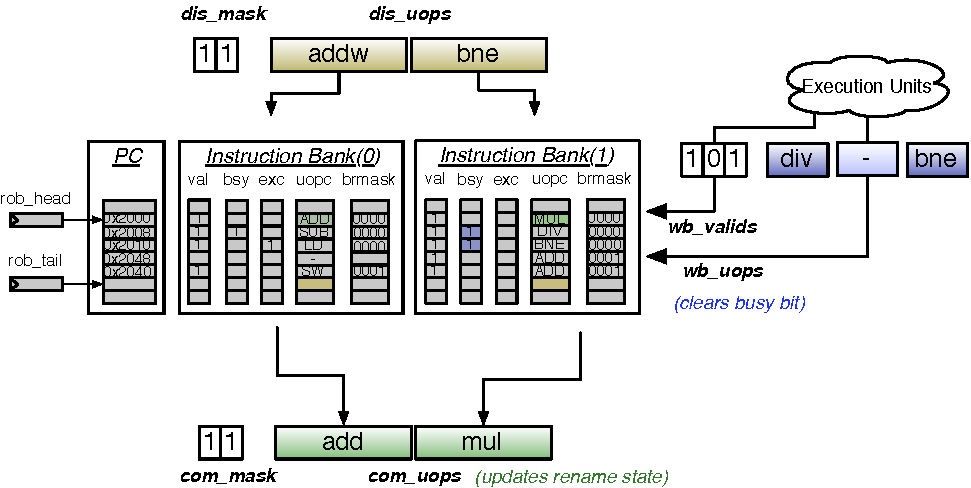
\includegraphics[scale =1] {figures/rob}}
	\caption{ \small The Reorder Buffer for a two-wide BOOM with three-issue. Dispatched uops ({\em dis\_uops}) are written at the bottom of the ROB ({\em rob\_tail}), while committed uops ({\em com\_uops}) are committed from the top, at {\em rob\_head}, and update the rename state. Uops that finish executing ({\em wb\_uops}) clear their {\em busy} bit. {\bf Note:} the dispatched uops are written into the same ROB row together, and are located consecutively in memory allowing a single PC to represent the entire row. }
	\label{fig:rob}
\end{figure}

\section{ROB State}

Each ROB entry contains relatively little state:

\begin{itemize}
\item is entry valid?
\item is entry busy?
\item is entry an exception?
\item branch mask (which branches is this entry still speculated under? 
\item rename state (what is the logical destination and the stale physical destination?)
\item floating-point status updates
\item other miscellaneous data (e.g., helpful for statistic tracking)
\end{itemize}

The PC and the branch prediction information is stored on a per-row basis (see Sec \ref{sec:pcstorage}).  The Exception State only tracks the oldest known excepting instruction (see Sec \ref{sec:rob_xcpt}). 

\subsection{Exception State}\label{sec:rob_xcpt}

The ROB tracks the oldest excepting instruction. If this instruction reaches the head of the ROB, then an exception is thrown. 

Each ROB entry is marked with a single-bit to signify whether or not the instruction has encountered exceptional behavior, but the additional exception state (e.g., the bad virtual address and the exception cause) is only tracked for the oldest known excepting instruction.  This saves considerable state by not storing this on a per entry basis. 

\subsection{PC Storage}\label{sec:pcstorage}

The ROB must know the PC of every inflight instruction.  This information is used in the following situations:

\begin{itemize}
\item Any instruction could cause an exception, in which the ``exception pc" (epc) must be known.
\item Branch and jump instructions need to know their own PC for for target calculation.
\item Jump-register instructions must know both their own PC {\bf and the PC of the following instruction} in the program to verify if the front-end predicted the correct JR target.
\end{itemize}

This information is incredibly expensive to store. Instead of passing PCs down the pipeline, branch and jump instructions access the ROB's ``PC File" during the {\em Register-read} stage for use in the Branch Unit. Two optimizations are used:


\begin{itemize}
\item only a single PC is stored per ROB row.\footnote{Because instructions within an ROB row are consecutive in the program, the instruction's ROB bank implicitly provides the lower PC bits.}
\item the PC File is stored in two banks, allowing a single read-port to read two consecutive entries simultaneously (for use with JR instructions).
\end{itemize}

\section{The Commit Stage}

When the instruction at the {\em commit head} is no longer busy (and it is not excepting), it may be committed and its changes to the architectural state of the machine made visible. For superscalar commit, the entire ROB row is analyzed for {\em not busy} instructions (and thus, up to the entire ROB row may be committed in a single cycle). The ROB will greedily commit as many instructions as it can per row to release resource as soon as possible. However, the ROB does not (currently) look across multiple rows to find commit-able instructions. 

Only once a store has been committed may it be sent to memory. For superscalar committing of stores, the LSU is told ``how many stores" may be marked as committed. The LSU will then drain the committed stores to memory as it sees fit. 

When an instruction (that writes to a register) commits, it then frees the {\em stale physical destination register}. The {\em stale pdst} is then free to be re-allocated to a new instruction. 


\section{Exceptions and Flushes}

Exceptions are handled when the instruction at the {\em commit head} is excepting. The pipeline is then flushed and the ROB emptied. The rename map tables must be reset to represent the true, non-speculative {\em committed} state. The front-end is then directed to the appropriate PC.  If an architectural exception, this is the {\em exception vector} as specified by the Control/Status Registers.  If it is a micro-architectural exception (e.g., a load/store ordering misspeculation) the failing instruction is refetched and execution can begin anew. 

\subsection{Parameterization - Rollback versus Single-cycle Reset}

The behavior of resetting the map tables is parameterizable.  The first option, as the only map table snapshots are for branches, is to rollback the ROB one row per cycle to unwind the rename state (this is the behavior of the MIPS R10k\cite{mipsr10k}).  For each instruction, the {\em stale physical destination} register is written back into the map table for its {\em logical destination} specifier. 

However, a faster single-cycle reset is available.  This is accomplished by using another rename snapshot that tracks the {\em committed} state of the rename tables. This {\em committed map table} is updated as instructions commit. 

\subsection{Causes}

The RV64G ISA provides relatively few exception sources:

\begin{quote}
\begin{description}
\item[Load/Store Unit] - page faults and memory ordering speculation errors
\item[Branch Unit] - misaligned fetches
\item[Decode Stage] - all other exceptions and interrupts can be handled before the instruction is dispatched to the ROB
\end{description}
\end{quote}

Note that memory ordering speculation errors are treated as exceptions, but actually only cause a pipeline ``retry". 
